%
% $Id: $
%
%
% Compilar a .pdf con LaTeX (pdflatex)
% Es necesario instalar Beamer (paquete latex-beamer en Debian)
%

%
% Gr�ficos:
% Los gr�ficos pueden suministrarse en PNG, JPG, TIF, PDF, MPS
% Los EPS deben convertirse a PDF (usar epstopdf)
%

\documentclass{beamer}
\usetheme{GSyC}
%\usebackgroundtemplate{\includegraphics[width=\paperwidth]{format/libresoft-bg.png}}
%\usepackage[spanish]{babel}
\usepackage[latin1]{inputenc}
\usepackage{graphics}
\usepackage{amssymb} % Simbolos matematicos

\ProcessOptions

%% Metadatos del PDF.
\hypersetup{
  pdftitle={Protocolos para la Transmisi�n de Audio y V�deo por Internet},
  pdfauthor={Gregorio Robles, Jes�s M. Gonz�lez Barahona},
  pdfcreator={GSyC, Universidad Rey Juan Carlos},
  pdfproducer=PDFLaTeX,
  pdfsubject={Protocolos para la Transmisi�n de Audio y V�deo por Internet},
}
%%

\begin{document}

\title{La \emph{shell} es tu amiga}
\subtitle{Protocolos para la Transmisi�n de Audio y V�deo en Internet}
\institute{\{grex,jgb\}@gsyc.urjc.es \\
GSyC, Universidad Rey Juan Carlos}
\author[Gregorio Robles, Jes�s M. Gonz�lez Barahona]{Gregorio Robles, Jes�s M. Gonz�lez Barahona}
\date[Nov 2014]{19 de noviembre de 2014}


\frame{
\maketitle
}


% Si el titulo o el autor se quieren acortar para los pies de p�gina
% se pueden redefinir aqu�:
%\title{Titulo corto}
%\author{Autores abreviado}


%% LICENCIA DE REDISTRIBUCION DE LAS TRANSPAS
\frame{
~
\vspace{4cm}

\begin{flushright}

\includegraphics[width=2.2cm]{figs/by-sa}

{\tiny
(cc) 2014 Gregorio Robles, Jes�s M. Gonz�lez Barahona \\
  Some rights reserved. This work licensed under Creative Commons \\
  Attribution-ShareAlike License. To view a copy of full license, see \\
\ \\
  http://creativecommons.org/licenses/by-sa/3.0/ or write to \\
  Creative Commons, 559 Nathan Abbott Way, Stanford, \\
  California 94305, USA. \\
\ 
}
\end{flushright}
}
%%

%-----------------------    ---------------------------------

\begin{frame}
\frametitle{Acortadores de teclado}

\begin{itemize}
   \item \texttt{Tab}: autocompleta programas, ficheros y directorios
   \item \texttt{Ctrl+A}: va al principio de la l�nea
   \item \texttt{Ctrl+E}: va al final de la l�nea
   \item \texttt{Ctrl+R}: busca por lo intrducido en la historia
   \item \texttt{Ctrl+K}: borra desde el punto actual al final
   \item \texttt{Ctrl+U}: borra hasta el punto actual
   \item \texttt{Ctrl+L}: \emph{aclara} la pantalla (como el mandato \texttt{clear})
   \item \texttt{Alt+F}: se mueve a la siguiente palabra
   \item \texttt{Alt+B}: se mueve a la palabra anterior
\end{itemize}

(algunos se pueden configurar en el propio terminal)


\end{frame}


%-----------------------    ---------------------------------

\begin{frame}
\frametitle{Uso de pesta�as}

\begin{center}
  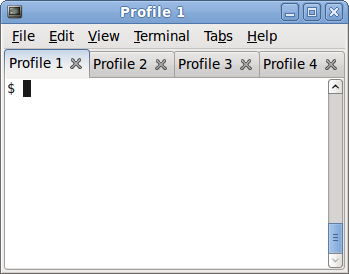
\includegraphics[width=4.5cm]{figs/tabs.png}
\end{center}


\begin{flushright}
{\tiny
http://unix.stackexchange.com/tags/gnome-terminal/info
}
\end{flushright}


\begin{itemize}
   \item Puedes poner nombre (t�tulo a cada pesta�a)
   \item Nueva pesta�a: \texttt{Ctrl+Alt+T} (yo lo suelo configurar como \texttt{Ctrl+T} para que sea igual que crear una nueva pesta�a en el navegador)
   \item Pesta�a siguiente/anterior: \texttt{Ctrl+PgUp} o \texttt{Ctrl+PgAbajo}
   \item \texttt{Alt+\emph{N}}: vas a la pesta�a \emph{N}
\end{itemize}


\end{frame}


%-----------------------    ---------------------------------

\begin{frame}
\frametitle{Procesos}

\begin{itemize}
   \item \texttt{top}: Muestra los procesos seg�n su \emph{consumo}
   \item \texttt{ps aux}: Lista todos los procesos del usuario
   \item \texttt{grep \emph{expr}}: Filtra por \emph{expr} 
   \item \texttt{ps aux | grep python}: Muestra la informaci�n de procesos que contengan \emph{python}
   \item \texttt{kill -9 \emph{pid}}: \emph{mata} el proceso con identificador \emph{pid}
\end{itemize}


\end{frame}


%-----------------------    ---------------------------------

\begin{frame}
\frametitle{Un peque�o chiste friqui para terminar}

\begin{center}
  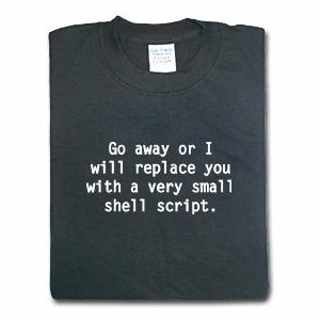
\includegraphics[width=7cm]{figs/shellscriptjoke.jpg}
\end{center}


\begin{flushright}
{\tiny
http://img819.imageshack.us/img819/4539/shellscriptjoke.jpg
}
\end{flushright}

\end{frame}

%-----------------------    ---------------------------------


\frame{
\maketitle
}

\end{document}
